%% BioMed_Central_Tex_Template_v1.06
%%                                      %
%  bmc_article.tex            ver: 1.06 %
%                                       %

%%IMPORTANT: do not delete the first line of this template
%%It must be present to enable the BMC Submission system to
%%recognise this template!!

%%%%%%%%%%%%%%%%%%%%%%%%%%%%%%%%%%%%%%%%%
%%                                     %%
%%  LaTeX template for BioMed Central  %%
%%     journal article submissions     %%
%%                                     %%
%%          <8 June 2012>              %%
%%                                     %%
%%                                     %%
%%%%%%%%%%%%%%%%%%%%%%%%%%%%%%%%%%%%%%%%%


%%%%%%%%%%%%%%%%%%%%%%%%%%%%%%%%%%%%%%%%%%%%%%%%%%%%%%%%%%%%%%%%%%%%%
%%                                                                 %%
%% For instructions on how to fill out this Tex template           %%
%% document please refer to Readme.html and the instructions for   %%
%% authors page on the biomed central website                      %%
%% http://www.biomedcentral.com/info/authors/                      %%
%%                                                                 %%
%% Please do not use \input{...} to include other tex files.       %%
%% Submit your LaTeX manuscript as one .tex document.              %%
%%                                                                 %%
%% All additional figures and files should be attached             %%
%% separately and not embedded in the \TeX\ document itself.       %%
%%                                                                 %%
%% BioMed Central currently use the MikTex distribution of         %%
%% TeX for Windows) of TeX and LaTeX.  This is available from      %%
%% http://www.miktex.org                                           %%
%%                                                                 %%
%%%%%%%%%%%%%%%%%%%%%%%%%%%%%%%%%%%%%%%%%%%%%%%%%%%%%%%%%%%%%%%%%%%%%

%%% additional documentclass options:
%  [doublespacing]
%  [linenumbers]   - put the line numbers on margins

%%% loading packages, author definitions

%\documentclass[twocolumn]{bmcart}% uncomment this for twocolumn layout and comment line below
\documentclass{bmcart}

%%% Load packages
%\usepackage{amsthm,amsmath}
%\RequirePackage{natbib}
\RequirePackage{hyperref}
\usepackage[utf8]{inputenc} %unicode support
%\usepackage[applemac]{inputenc} %applemac support if unicode package fails
%\usepackage[latin1]{inputenc} %UNIX support if unicode package fails


%%%%%%%%%%%%%%%%%%%%%%%%%%%%%%%%%%%%%%%%%%%%%%%%%
%%                                             %%
%%  If you wish to display your graphics for   %%
%%  your own use using includegraphic or       %%
%%  includegraphics, then comment out the      %%
%%  following two lines of code.               %%
%%  NB: These line *must* be included when     %%
%%  submitting to BMC.                         %%
%%  All figure files must be submitted as      %%
%%  separate graphics through the BMC          %%
%%  submission process, not included in the    %%
%%  submitted article.                         %%
%%                                             %%
%%%%%%%%%%%%%%%%%%%%%%%%%%%%%%%%%%%%%%%%%%%%%%%%%


%\def\includegraphic{}
%\def\includegraphics{}



%%% Put your definitions there:
\startlocaldefs
\setlength{\marginparwidth}{2cm}
%\usepackage[disable]{todonotes}
\usepackage[draft]{todonotes}
\endlocaldefs


%%% Begin ...
\begin{document}

%%% Start of article front matter
\begin{frontmatter}

\begin{fmbox}
\dochead{Data Note}

%%%%%%%%%%%%%%%%%%%%%%%%%%%%%%%%%%%%%%%%%%%%%%
%%                                          %%
%% Enter the title of your article here     %%
%%                                          %%
%%%%%%%%%%%%%%%%%%%%%%%%%%%%%%%%%%%%%%%%%%%%%%

\title{The old and grumpy biogas metagenome}

%%%%%%%%%%%%%%%%%%%%%%%%%%%%%%%%%%%%%%%%%%%%%%
%%                                          %%
%% Enter the authors here                   %%
%%                                          %%
%% Specify information, if available,       %%
%% in the form:                             %%
%%   <key>={<id1>,<id2>}                    %%
%%   <key>=                                 %%
%% Comment or delete the keys which are     %%
%% not used. Repeat \author command as much %%
%% as required.                             %%
%%                                          %%
%%%%%%%%%%%%%%%%%%%%%%%%%%%%%%%%%%%%%%%%%%%%%%

\author[
   addressref={cebitec,techfak},                   % id's of addresses, e.g. {aff1,aff2}
   corref={cebitec},                       % id of corresponding address, if any
%   noteref={n1},                        % id's of article notes, if any
   email={abremges@cebitec.uni-bielefeld.de}   % email address
]{\inits{AB}\fnm{Andreas} \snm{Bremges}}
\author[
   addressref={cebitec}
]{\inits{IM}\fnm{Irena} \snm{Maus}}
\author[
   addressref={cebitec}
]{\inits{AP}\fnm{Alfred} \snm{Pühler}}
\author[
   addressref={cebitec},
   noteref={n1}
]{\inits{AS}\fnm{Andreas} \snm{Schlüter}}
\author[
   addressref={cebitec,techfak},
%   corref={cebitec},
   noteref={n1},
   email={asczyrba@cebitec.uni-bielefeld.de}
]{\inits{AS}\fnm{Alexander} \snm{Sczyrba}}

%%%%%%%%%%%%%%%%%%%%%%%%%%%%%%%%%%%%%%%%%%%%%%
%%                                          %%
%% Enter the authors' addresses here        %%
%%                                          %%
%% Repeat \address commands as much as      %%
%% required.                                %%
%%                                          %%
%%%%%%%%%%%%%%%%%%%%%%%%%%%%%%%%%%%%%%%%%%%%%%

\address[id=cebitec]{%                           % unique id
  \orgname{Center for Biotechnology, Bielefeld University}, % university, etc
  %\street{},                     %
  %\postcode{33615}                                % post or zip code
  %\city{Bielefeld},                              % city
  \cny{Germany}                                    % country
}
\address[id=techfak]{%
  \orgname{Faculty of Technology, Bielefeld University},
  %\street{},
  %\postcode{}
  %\city{Bielefeld},
  \cny{Germany}
}

%%%%%%%%%%%%%%%%%%%%%%%%%%%%%%%%%%%%%%%%%%%%%%
%%                                          %%
%% Enter short notes here                   %%
%%                                          %%
%% Short notes will be after addresses      %%
%% on first page.                           %%
%%                                          %%
%%%%%%%%%%%%%%%%%%%%%%%%%%%%%%%%%%%%%%%%%%%%%%

\begin{artnotes}
%\note{Sample of title note}     % note to the article
\note[id=n1]{Equal contributor} % note, connected to author
\end{artnotes}

\end{fmbox}% comment this for two column layout

%%%%%%%%%%%%%%%%%%%%%%%%%%%%%%%%%%%%%%%%%%%%%%
%%                                          %%
%% The Abstract begins here                 %%
%%                                          %%
%% Please refer to the Instructions for     %%
%% authors on http://www.biomedcentral.com  %%
%% and include the section headings         %%
%% accordingly for your article type.       %%
%%                                          %%
%%%%%%%%%%%%%%%%%%%%%%%%%%%%%%%%%%%%%%%%%%%%%%

\begin{abstractbox}

\begin{abstract} % abstract
\parttitle{Background}
a presentation of the interest or relevance of these data for the broader community
%
\parttitle{Findings}
a very brief preview of the data type(s) produced, the methods used, and information relevant to data validation
%
\parttitle{Conclusions}
a short summary of the potential uses of these data and implications for the field
\end{abstract}

%%%%%%%%%%%%%%%%%%%%%%%%%%%%%%%%%%%%%%%%%%%%%%
%%                                          %%
%% The keywords begin here                  %%
%%                                          %%
%% Put each keyword in separate \kwd{}.     %%
%%                                          %%
%%%%%%%%%%%%%%%%%%%%%%%%%%%%%%%%%%%%%%%%%%%%%%

\begin{keyword}
\kwd{Biogas}
\kwd{Metagenome}
\kwd{Sequencing}
\kwd{Assembly}
\kwd{Annotation}
\end{keyword}

% MSC classifications codes, if any
%\begin{keyword}[class=AMS]
%\kwd[Primary ]{}
%\kwd{}
%\kwd[; secondary ]{}
%\end{keyword}

\end{abstractbox}
%
%\end{fmbox}% uncomment this for twcolumn layout

\end{frontmatter}

%%%%%%%%%%%%%%%%%%%%%%%%%%%%%%%%%%%%%%%%%%%%%%
%%                                          %%
%% The Main Body begins here                %%
%%                                          %%
%% Please refer to the instructions for     %%
%% authors on:                              %%
%% http://www.biomedcentral.com/info/authors%%
%% and include the section headings         %%
%% accordingly for your article type.       %%
%%                                          %%
%% See the Results and Discussion section   %%
%% for details on how to create sub-sections%%
%%                                          %%
%% use \cite{...} to cite references        %%
%%  \cite{koon} and                         %%
%%  \cite{oreg,khar,zvai,xjon,schn,pond}    %%
%%  \nocite{smith,marg,hunn,advi,koha,mouse}%%
%%                                          %%
%%%%%%%%%%%%%%%%%%%%%%%%%%%%%%%%%%%%%%%%%%%%%%

%%%%%%%%%%%%%%%%%%%%%%%%% start of article main body
% <put your article body there>

\section*{Data description}
%
\subsection*{Background}
Biogas important energy source. Clean and awesome.
Number of biogas plants in Germany/Europe/worldwide.
Key is process optimization, not building more and more plants.
Little is known about the microbial community responsible for everything\todo{section not final!}.

Here, we report the first deeply sequenced metagenome (and metatranscriptome?) of an agricultural production-scale biogas plant on the Illumina platform \cite{GigaScience}.
We sequenced $27.3 \times$ and $19.3 \times$ deeper than previous studies relying on 454 \cite{Jaenicke2011} or SOLiD \cite{Wirth2012} sequencing\todo{phrasing}.
%454 \cite{Jaenicke2011}: 1,963,716 reads, 843,091,863 bases: factor of 27.3 more
%SOLiD \cite{Wirth2012}: 23,897,590 reads, 1,194,879,500 bases: factor of 19.3 more
%No idea about the 454 data from Solli, 2014: http://www.ncbi.nlm.nih.gov/bioproject/?term=PRJNA261310
These data will enable a deeper exploration of the biogas-producting microbial community, a key step towards process optimization.
%
\subsection*{Digester management}
The biogas plant, located in North Rhine Westphalia, Germany, features a mesophilic continuous wet fermentation technology and was designed for a capacity of $537\,kW_{el}$ combined heat and power (CHP) generation.
The process comprises two digesters: a primary digester, where biogas and methane is produced, and a secondary digester, insignificant for production.
The primary digester is fed hourly with a mixture of maize silage and liquid pig manure.
The biogas and methane yields at the time of sampling were at $810.5$ and $417.8$ liters per kg organic dry matter ($l / kg\,oDM$), respectively.
After a theoretical retention time of $55$ days, the digestate is stored in the closed, non-heated final storage tank.
Further metadata are summarized in Table \ref{tBiogasPlant}.
%
\subsection*{Sampling and DNA isolation}
Samples from the primary digester of the aforementioned biogas plant were taken in November 2010.
Prior to sampling process, approximately $15\,L$ of fermenter substrate were discarded before aliquots of $1\,L$ were transferred into clean gastight sampling vessels and transported directly to the laboratory.

A $20\,g$ aliquot of the fermentation sample was used for total community DNA preparation as described previously \cite{Schlueter2008}.
%
\subsection*{Metagenomic sequencing}
In total, we sequenced four different metagenome shotgun libraries with different insert sizes, resulting in over $23$ gigabases scattered across $144$ million reads.\todo{we need actual numbers somewhere}
On Illumina's Genome Analyzer IIx system, we sequenced two libraries with an average insert size of $250\,nt$ and $450\,nt$, respectively, applying the Paired-End DNA Sample Preparation Kit (Illumina Inc.) as described by the manufacturer.
On Illumina's MiSeq system, we sequenced two further libraries with an average insert size of $190\,nt$ and $690\,nt$, respectively, applying the Nextera DNA Sample Preparation Kit (Illumina Inc.) as described by the manufacturer.
In all cases, we sequenced for approximately 300 cycles, applying the $2 \times 150\,nt$ paired-end protocol.\todo[inline]{Eher kein 2x250: MiSeq v2 öffentlich 10/2012, Alex und ich hatten die MiSeq Daten in 07/2012!}
%Two metagenome shotgun libraries were prepared with the average insert size of 690 nt and 190 nt, respectively, applying the Nextera DNA Sample Preparation Kit (Illumina Inc.) according to the manufacturer's instructions. The libraries were sequenced applying the 2 x 250 nt paired-end protocol on the Illumina MiSeq platform.
%Additionally, two further metagenome shotgun libraries were constructed with the average insert size of 450 nt and 250 nt, respectively, applying the Paired-end Sample Preparation Kit (Illumina Inc.) as described by the manufacturer. Prepared libraries were sequenced applying 2 x 150 nt paired-end protocol on the Illumina Genome Analyzer IIx instrument.
%
\subsection*{Sequence quality control}
Quality control with FastQC, version 0.11.2\todo{cite if needed}. Adapter contamination in Lane 7\todo{mention at all?}.

We used Trimmomatic \cite{Trimmomatic}, version 0.32, for adapter removal and moderate quality trimming.
After adapter clipping, using Trimmomatic's \emph{Truseq2-PE} and \emph{Nextera-PE} templates, we removed leading and trailing low quality bases (below quality 3).
Then, we performed an adaptive quality trimming, balancing read length against error rate (target read length of 100 bases, strictness of 0.2, thus favouring read length over error sensitivity).
Finally, reads shorter than $36$ bases were discarded.

Either another table or brief summary post-QC\todo{section not final!}.
%
\subsection*{Metagenome assembly and quality assessment}
We assembled the metagenome with Ray Meta \cite{RayMeta}, version 2.3.0\todo{2.3.1}, using a $k$-mer size of $31$ and a minimum contig length of $1,000\,bp$.
This resulted in a total assembly size of approximately $217$ megabases in $55,563$ contigs, with an N50 value of $8,137\,bp$.
Table \ref{tAssembly} summarizes our results.

We aligned the post-QC sequencing reads to the assembled contigs with bowtie2 \cite{Bowtie2}, version 2.2.1\todo{2.2.4}, and used samtools \cite{Samtools}, version 1.1, to convert SAM to BAM and thereafter sort the alignment file.\todo{Run LAP or ALE}
%
\subsection*{Gene prediction and annotation}
We then used MetaProdigal \cite{MetaProdigal}, version 2.6.1, to predict $239,412$ protein-coding genes on the assembled contigs. Table \ref{tGenes} also includes these results.

We blasted all predicted genes against the KEGG database \cite{KeggDB}, release 72.0, using Protein-Protein BLAST \cite{BlastPlus}, version 2.2.29+. 
Of the $239,412$ predicted genes, $230,354$ were found in the KEGG database.
We determined the KEGG Orthology (KO) for each gene by mapping the top-scoring BLAST hit to its KO.

\subsection*{Coverage analysis}
We counted aligned reads in predicted genes with HTSeq \cite{HTSeq}, version 0.6.1p1\todo{0.6.1p2}.
Figure \ref{fCoverage} relates the metagenome and the metatranscriptome.\todo{work in progress and up for discussion}
%It was generated with the ggplot2 package (cite) in R (cite).
%
\section*{Availability}
\subsection*{Data accession}
The datasets supporting the results of this article are available in the [repository name] repository, [unique persistent identifier and hyperlink to datasets in http:// format].
%
\subsection*{Reproducibility}
The complete workflow is organized in a single GNU Makefile and available on GitHub \cite{GitHub}.
Starting from the raw read files, available from SRA and/or GigaDB, all data and results can be reproduced by a simple invocation of \emph{make}.
Excluding KEGG analysis, which relies on a commercial license \todo{phrasing} of the KEGG database, all steps are performed using free and open-source software.
%It might be needed to adjust some paths to the used tools and databases, or alternatively symlink everything in the working directory.
%
\subsection*{Requirements}
The assembly of the metagenome data sets with Ray Meta requires 70 GB of RAM. Using only 40 cores, it completed within 12 hours wall-clock time.
Annotation with blast took, of course, forever.\todo{log runtime and memory in final run!}
%
\section*{Discussion}
Potential use cases.
Metagenomic (and metatranscriptomic?) profiling of the biogas-producing microbial community.
Identification of metaproteomic data out there (cite Vera, in preparation).

Ultimate goal: process optimization by biological insights\todo{section not final!}.

%%%%%%%%%%%%%%%%%%%%%%%%%%%%%%%%%%%%%%%%%%%%%%
%%                                          %%
%% Backmatter begins here                   %%
%%                                          %%
%%%%%%%%%%%%%%%%%%%%%%%%%%%%%%%%%%%%%%%%%%%%%%

%Remove \newpage
\newpage
\begin{backmatter}

\section*{Competing interests}
The authors declare that they have no competing interests.

\section*{Author's contributions}
AB conveived and performed all bioinformatic analyses and wrote the paper.
IM investigated all metadata and drafted part of the data description.
AP, ASch and will do something at some point.
AScz conveived of many of the analyses and revised the paper.
ASch and AScz jointly directed the project.
All authors read and approved the final manuscript.

\section*{Acknowledgements}
AB and IM are supported by a fellowship from the CLIB Graduate Cluster Industrial Biotechnology.\todo{Funding Andreas S, Stadtwerke?}

%%%%%%%%%%%%%%%%%%%%%%%%%%%%%%%%%%%%%%%%%%%%%%%%%%%%%%%%%%%%%
%%                  The Bibliography                       %%
%%                                                         %%
%%  Bmc_mathpys.bst  will be used to                       %%
%%  create a .BBL file for submission.                     %%
%%  After submission of the .TEX file,                     %%
%%  you will be prompted to submit your .BBL file.         %%
%%                                                         %%
%%                                                         %%
%%  Note that the displayed Bibliography will not          %%
%%  necessarily be rendered by Latex exactly as specified  %%
%%  in the online Instructions for Authors.                %%
%%                                                         %%
%%%%%%%%%%%%%%%%%%%%%%%%%%%%%%%%%%%%%%%%%%%%%%%%%%%%%%%%%%%%%

% if your bibliography is in bibtex format, use those commands:
\bibliographystyle{bmc-mathphys} % Style BST file
\bibliography{bremges_gigascience_2014}      % Bibliography file (usually '*.bib' )
\todo{Less author names, remove PMC?}
% or include bibliography directly:
% \begin{thebibliography}
% \bibitem{b1}
% \end{thebibliography}

%%%%%%%%%%%%%%%%%%%%%%%%%%%%%%%%%%%
%%                               %%
%% Figures                       %%
%%                               %%
%% NB: this is for captions and  %%
%% Titles. All graphics must be  %%
%% submitted separately and NOT  %%
%% included in the Tex document  %%
%%                               %%
%%%%%%%%%%%%%%%%%%%%%%%%%%%%%%%%%%%

%%
%% Do not use \listoffigures as most will included as separate files

%Remove \newpage
\newpage
\section*{Figures}
\begin{figure}[h!]
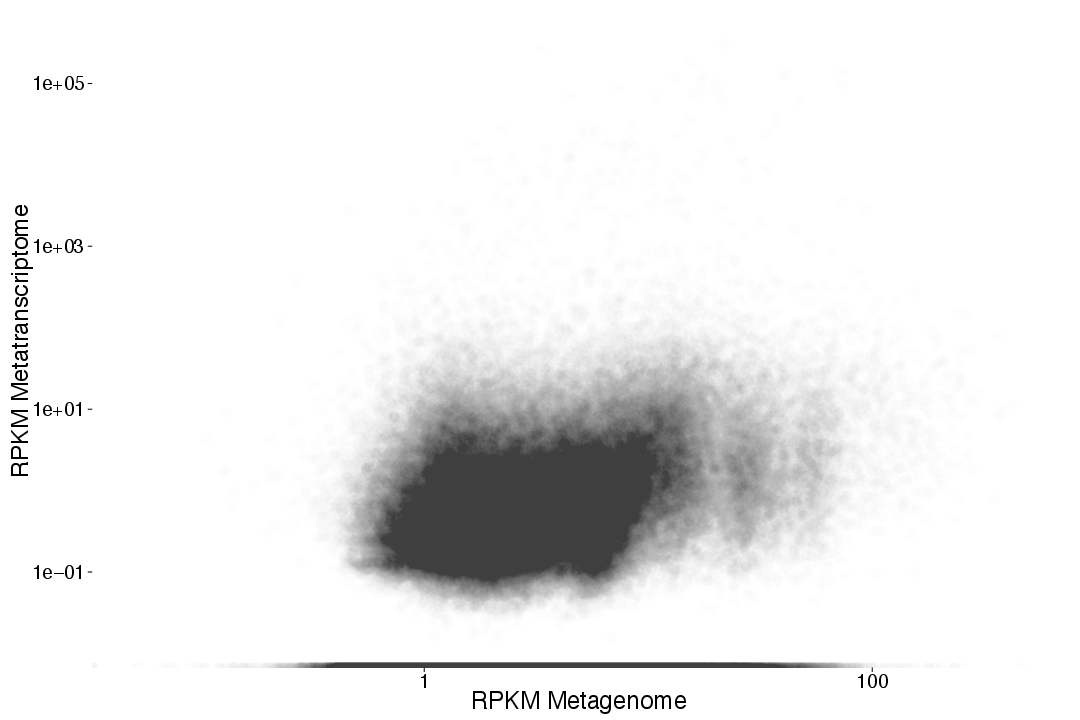
\includegraphics[width=\textwidth]{Rplot}
\caption{\csentence{Relating the metagenome and metatranscriptome.} FPKM values, can discuss and decide once results are ready. I intend to highlight all genes involved in the methane metabolism (\href{http://www.genome.jp/kegg-bin/show_pathway?org_name=ko&mapno=00680&mapscale=&show_description=hide}{path:ko00680}). Low-quality image as a placeholder.}
\label{fCoverage}
\end{figure}
%
%\begin{figure}[h!]
%\caption{\csentence{Sample figure title.} Figure legend text.}
%\end{figure}

%%%%%%%%%%%%%%%%%%%%%%%%%%%%%%%%%%%
%%                               %%
%% Tables                        %%
%%                               %%
%%%%%%%%%%%%%%%%%%%%%%%%%%%%%%%%%%%

%% Use of \listoftables is discouraged.
%%

%Remove \newpage
\newpage
\section*{Tables}
\begin{table}[h!]
\caption{Characteristics of the studied biogas plant. Primary digester, sampling date: Nov 15, 2010.}
\begin{tabular}{rl}
\hline
Process parameter & Sample\\
\hline
Net volume & $2041\,m^{3}$\\
Dimensions & $6.4\,m$ high, diameter of $21\,m$\\
Electrical capacity & $537\,kW_{el}$\\
\hline
pH & $7.83$\\
Temperature & $40\,^{\circ}{\rm C}$\\
Conductivity & $22.10\,mS/cm$\\
Volative organic acids (VOA) & $5327\,mg/l$\\
Total inorganic carbon (TIC) & $14397\,mg/l$\\
VOA/TIC & $0.37$\\
Ammoniacal nitrogen & $2.93\,g/l$\\
Acetic acid & $863\,mg/l$\\
Propionic acid & $76\,mg/l$\\
\hline
Fed substrates & $72\,\%$ maize silage, $28\,\%$ pig manure\\
Organic load & $4.0\,kg\,oDM\,m^{-3}\,d^{-1}$\\
Biogas yield & $810.5\,l/kg\,oDM$\\
Methane yield & $417.8\,l/kg\,oDM$\\
\hline
\end{tabular}
\label{tBiogasPlant}
\end{table}
\todo{TIC only calculated, might be a few digits off}

\begin{table}[h!]
\caption{Metagenome assembly. Some assembly statistics, minimum contig size of $1,000\,bp$.}
\begin{tabular}{rl}
\hline
Assembly metric & Our assembly\\
\hline
Total size & $216,554,757\,bp$\\
Number of contigs & $55,563$\\
N50 value & $8,137\,bp$\\
Largest contig & $319,083\,bp$\\
\hline
\end{tabular}
\label{tAssembly}
\end{table}

\begin{table}[h!]
\caption{Gene prediction and annotation. Whatever.}
\begin{tabular}{rl}
\hline
Annotation metric & Our annotaion\\
\hline
Predicted genes & $239,412$\\
of these, full-length & $160,124\,(66.9\,\%)$\\
KEGG stuff & ?\\
\hline
\end{tabular}
\label{tGenes}
\end{table}

%%%%%%%%%%%%%%%%%%%%%%%%%%%%%%%%%%%
%%                               %%
%% Additional Files              %%
%%                               %%
%%%%%%%%%%%%%%%%%%%%%%%%%%%%%%%%%%%

%\section*{Additional Files}
%  \subsection*{Additional file 1 --- Sample additional file title}
%    Additional file descriptions text (including details of how to
%    view the file, if it is in a non-standard format or the file extension).  This might
%    refer to a multi-page table or a figure.
%
%  \subsection*{Additional file 2 --- Sample additional file title}
%    Additional file descriptions text.


\end{backmatter}
%Remove \newpage and \listoftodos
\newpage
\listoftodos
\end{document}
